
\chapter{Koncepcja i projekt systemu}

\label{chap:concept}Proponowany model programowania miał być jak
najbardziej naturalny dla programistów zaznajomionych z zagadnieniami
programowania równoległego (por. \ref{sec:background-rownolegle})
i korzystać z koncepcji wątków, pamięci rozproszonej oraz zamków.
Wprowadzone abstrakcje wysokiego poziomu miały na celu ukrycie przed
użytkownikiem leżącego u podstaw programowania rozproszonego (por.
\ref{sec:background-Przetwarzanie-rozproszone}) mechnizmu przesyłania
komunikatów. 


\section{Komunikacja}

\label{sub:concept-Komunikacja}Każdy z węzłów (def. \ref{def:background-Wezel-obliczeniowy})
w klastrze (def. \ref{def:background-Klaster}) może komunikować\ się
poprzez sieć z każdym innym węzłem. Przyjęto następujące założenia
co do protokołów komunikacyjnych:
\begin{enumerate}
\item protokół zastosowany w warstwie transportowej powinien zapewnić niezawodne
dostarczenie wszystkich wiadomości,
\item protokół działający w warstwie aplikacji powinien oczekiwać odpowiedzi
na wysyłane żądania. 
\end{enumerate}
Nie jest wymagane zachowanie kolejności dostarczania wiadomości --
w szczególności z uwagi na to, że w kanale znajduje się w danym momencie
co najwyżej jedna wiadomość. Dla uzyskania transparentności procesu
rozpraszania obliczeń sam proces przesyłania komunikatów pomiędzy
węzłami jest ukryty przed użytkownikiem.

Zakładamy również, że bezpieczeństwo klastra opiera się na tym, iż
działa on w~odseparowanej sieci, tj. bez bezpośredniego dostępu z
sieci publicznej (internetu). W związku z tym zastosowane protokoły
komunikacyjne nie muszą zapewniać mechanizmów uwierzytelniania i autoryzacji.
\begin{defn}
~

\noindent \label{def:background-Wezel-obliczeniowy}Mianem \dcsstrong{węzła obliczeniowego}
(w skrócie: \dcsstrong{węzła}) określamy komputer, na którym działa
usługa zaimplementowana z użyciem biblioteki Bluepath, której celem
jest zlecanie bądź wykonanie zleconych zadań.
\end{defn}
Klaster systemu Bluepath składa się z węzłów obliczeniowych połączonych
siecią. Rysunek \ref{fig:background-schemat-systemu} przedstawia
schemat architektury systemu.
\begin{defn}
~

\noindent \label{def:background-Klaster}\dcsstrong{Klaster} to zbiór
węzłów obliczeniowych, które są zarejestrowane we wspólnej \dcsname{usłudze odnajdywania węzłów}
(def. \ref{def:background-Usluga-odnajdywania-wezlow}).
\end{defn}
\begin{figure}
\centering{}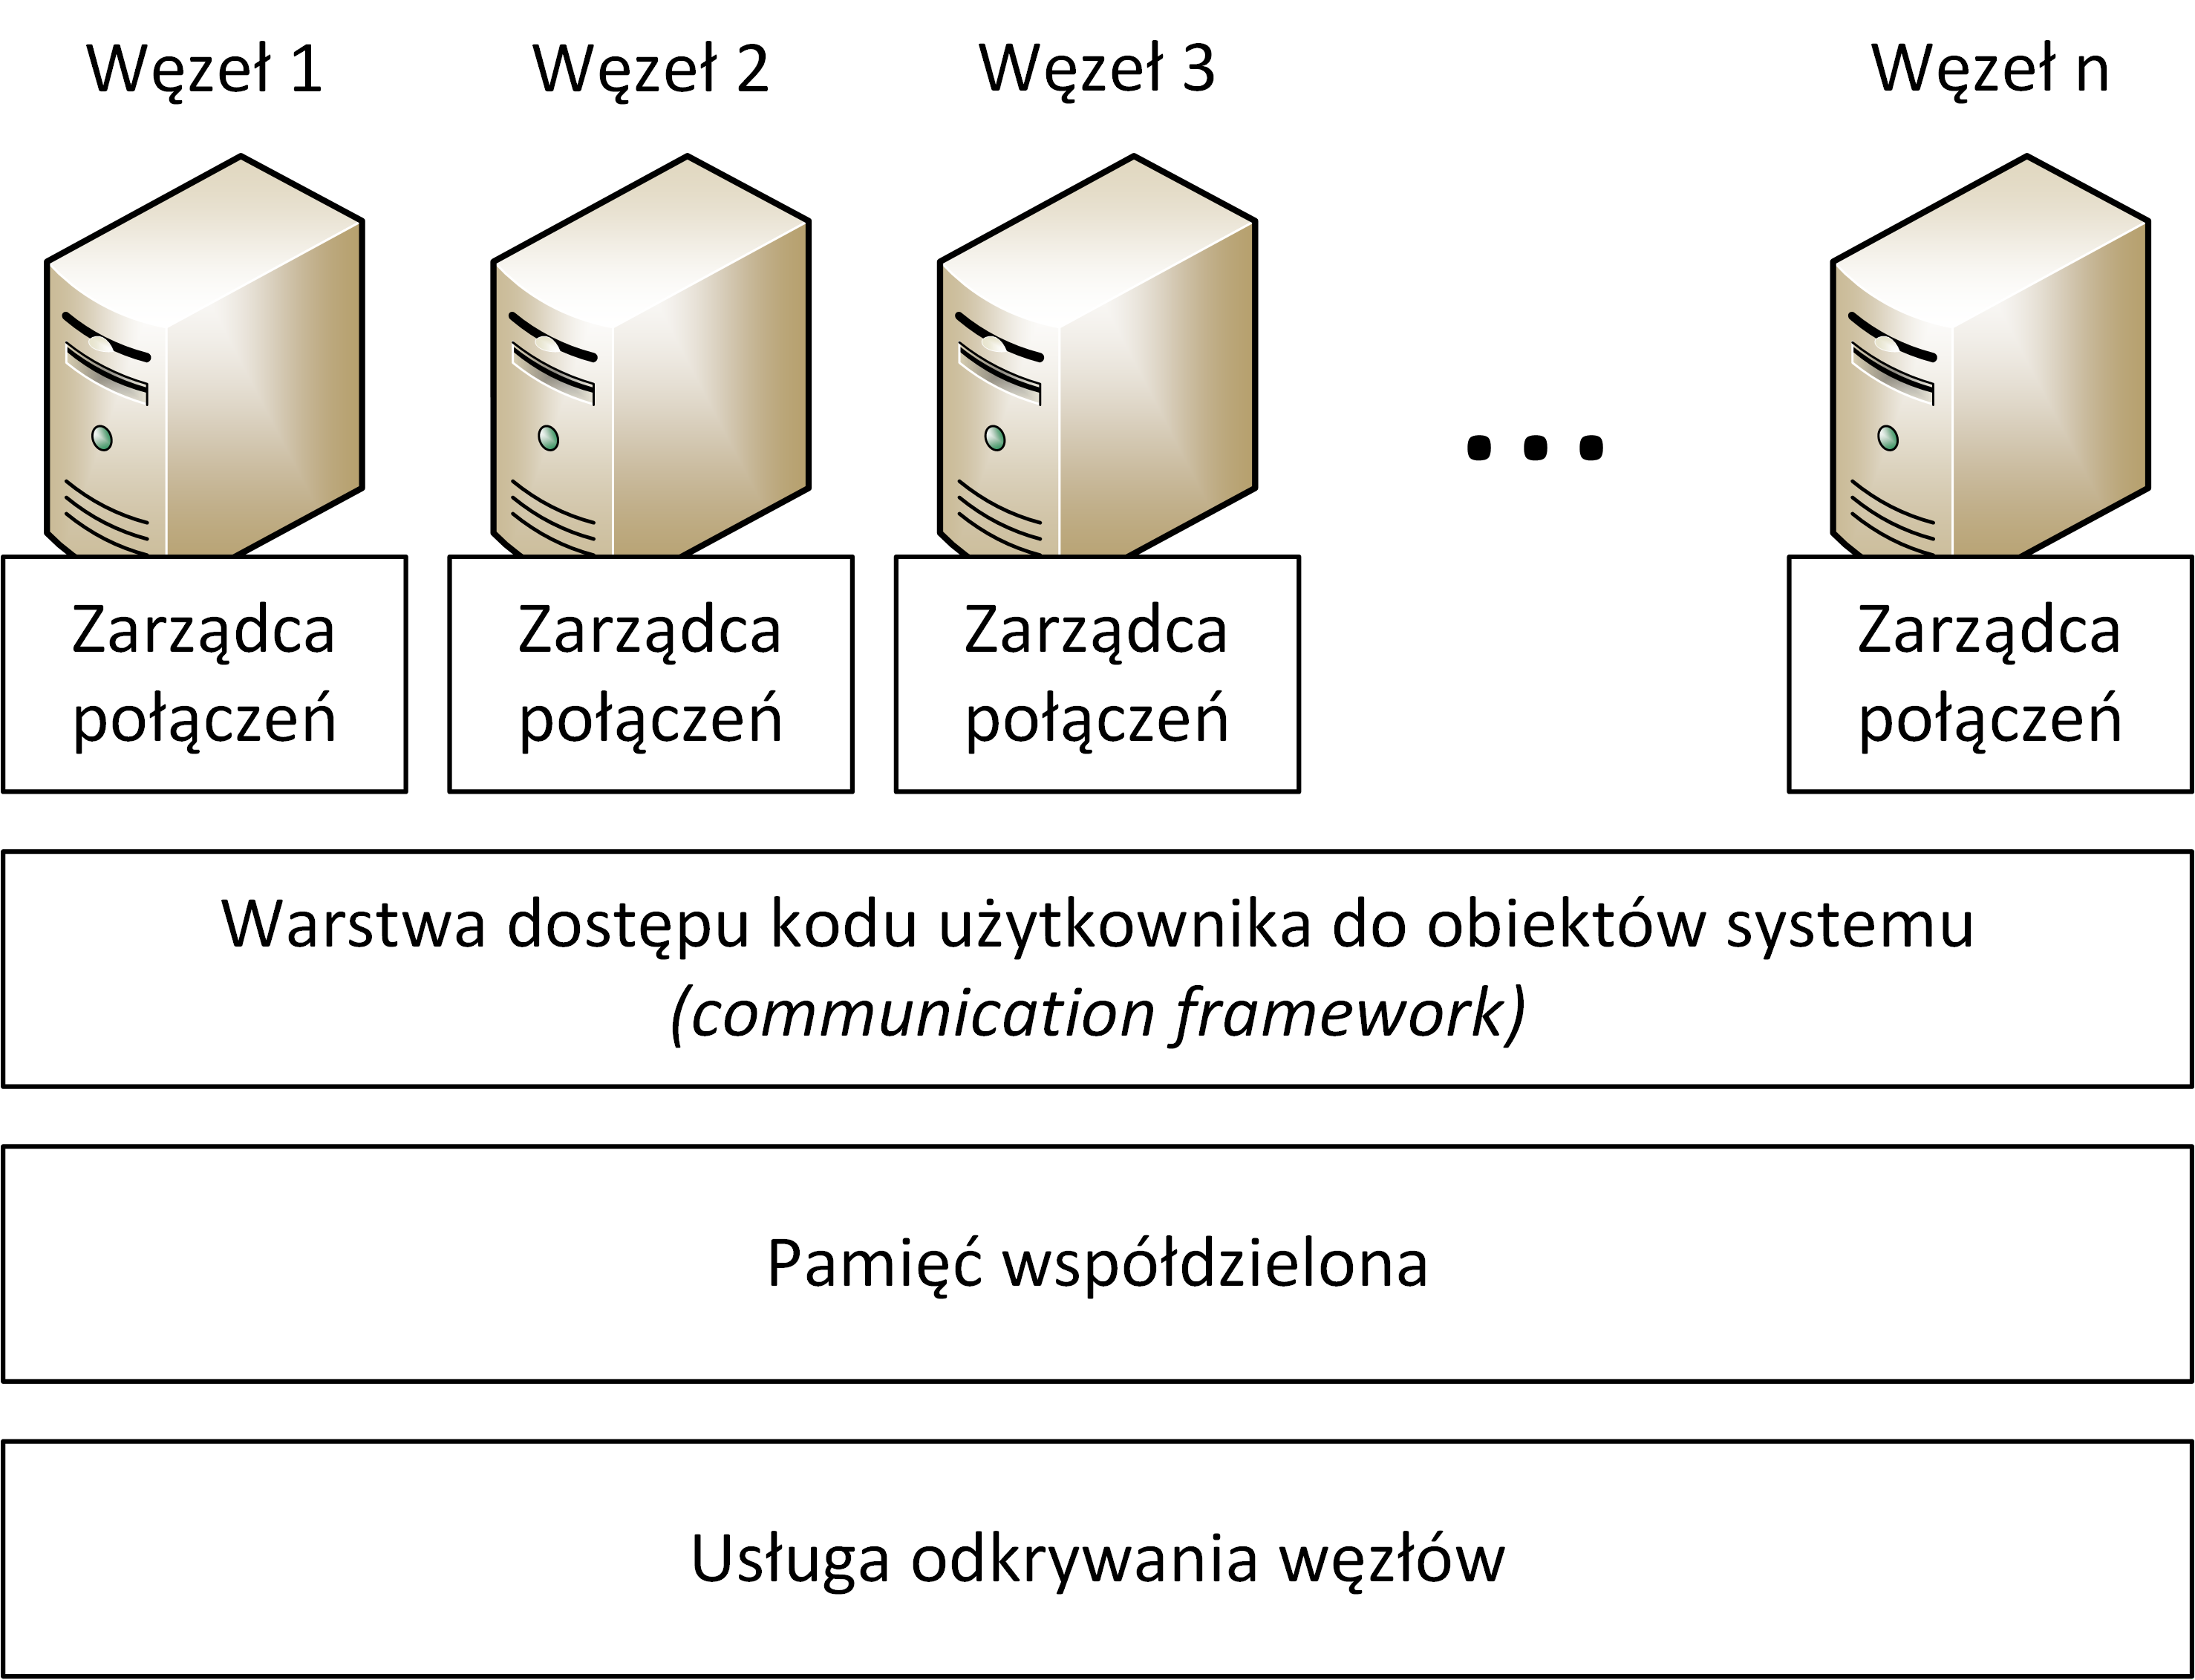
\includegraphics[scale=0.85]{images/schemat-systemu}\protect\caption{\label{fig:background-schemat-systemu}Schemat architektury systemu}
\end{figure}



\section{Usługa odnajdywania węzłów}

Jednym z podstawowych założeń jest posiadanie przez wszystkie węzły
w systemie lokalnej wiedzy o wszystkich innych węzłach obecnych w
klastrze. Informacje dotyczące stanu poszczególnych węzłów są dostarczane
przez \dcsname{usługę odnajdywania węzłów}. Usługa ta powinna
obsługiwać sytuację rejestracji oraz wyrejestrowania się węzłów. System
z założenia abstrahuje od sposobu realizacji tej usługi (czy będzie
to system scentralizowany, czy rozproszony np. oparty na algorytmie
plotkującym). W związku z pełnioną rolą, \dcsname{usługa odnajdywania węzłów}
jest kluczowym elementem przy implementacji wykrywania awarii węzłów
w klastrze. Nowe węzły muszą zarejstrować się w usłudze. Po rejestracji
są one monitorowane dopóki nie opuszczą klastra i wyrejestrują się
lub ulegną awarii. Niedostępne węzły -- tzn. takie, które nie odpowiedziały
na zapytanie w określonym czasie -- są usuwane z klastra.
\begin{defn}
~

\noindent \label{def:background-Usluga-odnajdywania-wezlow}\dcsstrong{Usługa odnajdywania węzłów}
to system umożliwiający węzłom odnajdywanie się wzajemnie w sieci
i łączenie w klaster obliczeniowy.
\end{defn}

\subsection{Zarządca połączeń}

Każdy węzeł powinien przechowywać lokalnie obraz klastra, aby w momencie,
kiedy zajdzie potrzeba zlecenia zadania jednemu ze \dcsname{zdalnych wykonawców}
nie musiał odpytywać \dcsname{usługi odnajdywania węzłów}. Tym
zadaniem zajmuje się \dcsname{zarządca połączeń}. Przechowuje
on też dodatkowe informacje, które mogą zostać wykorzystane przez
\dcsname{planistę}, takie jak statystyki obciążenia węzłów.
\begin{defn}
~

\noindent \dcsstrong{Zarządca połączeń} to klient usługi odnajdywania
węzłów, który odpowiada za rejestrowanie, wyrejestrowywanie i przechowywanie
lokalnego obrazu stanu klastra na każdym z węzłów.
\end{defn}

\section{Wątek rozproszony}

Specyfika systemu Bluepath wymaga rozróżnienia wątku systemu operacyjnego
oraz \dcsname{wątku rozproszonego} rozumianego jako jednostki przetwarzania
w systemie. \dcsname{Wątek rozproszony} jest tworzony na podstawie
statycznej metody, która przyjmuje dowolną, liczbę parametrów i zwraca
wartość. Wynik przechwytywany jest przez środowisko i udostępniany
do odczytu na węźle, który zlecił wykonanie wątku. Rozproszony wątek
może zostać wykonany na dowolnym węźle obliczeniowym oraz uruchamiać
kolejne rozproszone wątki. Decyzja o wyborze miejsca wykonania wątku
podejmowana jest z wykorzystaniem lokalnej wiedzy o stanie klastra
przez \dcsname{planistę}. Wątek rozproszony musi wykonać się w całości
na jednym z węzłów -- nie ma możliwości wstrzymania przetwarzania,
przeniesienia wątku razem z aktualnym stanem i~wznowienia obliczeń
na innym węźle.
\begin{defn}
~

\noindent \label{def:background-Rozproszony-watek}\dcsstrong{Wątek rozproszony}
reprezentuje jednostkę przetwarzania w systemie. Opakowuje fragment
kodu, który może być wykonany na dowolnym węźle obliczeniowym.
\end{defn}

\subsection{Problem detekcji zakończenia}

W punkcie \ref{sub:background-Problem-detekcji-zakonczenia} zasygnalizowano
konieczność zaproponowania rozwiąznia problemu detekcji zakończenia.
\dcsname{Wątki rozproszone} tworzą drzewiastą strukturę przetwarzania
-- można ją określić mianem modelu dyfuzyjnego. Wyróżniamy tutaj inicjatora
przetwarzania w korzeniu logicznego drzewa oraz jego następniki --
procesy potomne, które ponadto mogą inicjować kolejne procesy. Użytkownik
musi zapewnić, że proces-rodzic nie zakończy się, dopóki nie zakończą
się jego procesy-dzieci korzystając z przeznaczonej do tego metody.


\section{Wykonawca}

W celu ograniczenia liczby zadań pełnionych przez \dcsname{wątek rozproszony}
zdefiniowano \dcsname{wykonawcę} -- element odpowiedzialny za wykonywanie
wątków. Zastosowanie takiej abstrakcji pozwala potraktować przetwarzanie
lokalne oraz zdalne w podobny sposób. Specjalizacje -- \dcsname{lokalny wykonawca}
i \dcsname{zdalny wykonawca} -- wynikają z potrzeby realizacji innej
logiki w przypadku wykonania kodu na lokalnej i zdalnej maszynie. 


\subsection{Lokalny wykonawca}

Wszystkie wątki wykonywane lokalnie (zarówno te które pochodzą z lokalnego
węzła jak i te zlecone przez inny węzeł) są zarządzane przez \dcsname{lokalnych wykonawców}.
Do zadań \dcsname{lokalnego wykonawcy} należą:
\begin{itemize}
\item rozpoczęcie przetwarzania, 
\item przekierowanie parametrów, 
\item przechwycenie wyjątków,
\item udostępnienie wyników wyższym warstwom po zakończeniu przetwarzania.\end{itemize}
\begin{defn}
~

\noindent \dcsstrong{Lokalny wykonawca} to obiekt, który odpowiada
za faktyczne wykonanie otrzymanego zadania.
\end{defn}

\subsection{Zdalny wykonawca}

Reprezentacją zdalnego uruchomienia \dcsname{wątku rozproszonego}
jest obiekt \dcsname{zdalnego wykonawcy}. Zleca on wykonanie zadania
węzłowi wybranemu przez \dcsname{planistę} oraz monitoruje stan
wykonania zadania (zakończenie, wystąpienie błędów). Jest on również
odpowiedzialny za odebranie wyniku przetwarzania i udostępnienie go
do odczytu na węźle zlecającym zadanie.
\begin{defn}
~

\noindent \dcsstrong{Zdalny wykonawca} to obiekt, który odpowiada
za zlecenie wykonania zadania na zdalnej maszynie.
\end{defn}

\section{Planista}

Elementem systemu decydującym o wyborze miejsca wykonywania \dcsname{wątku rozproszonego}
jest \dcsname{planista}. Każda jego realizacja musi być oparta na
zdefiniowanym interfejsie. Dzięki temu użytkownik może przygotować
własną implementację \dcsname{planisty} dostosowaną do prowadzonego
przetwarzania lub wybrać jedną z dostarczonych razem z biblioteką.
\begin{defn}
~

\noindent \dcsstrong{Planista} odpowiada za wybór węzła, do którego
wysłane zostanie zlecenie wykonania zadania. Realizuje zdefiniowaną
strategię szeregowania zadań w klastrze.
\end{defn}

\section{Pamięć rozproszona}

\label{sec:concept-Rozproszona-pami=000119=000107-wsp=0000F3=000142dzielona}Często
w ramach przetwarzania rozproszonego zachodzi potrzeba przesyłania
danych między węzłami. W celu jej zrealizowania, jako część biblioteki
\dcsname{Bluepath}, dostarczana jest abstrakcja \dcsname{pamięci rozproszonej}.
Umożliwia ona synchronizację i wymianę danych między działającymi
wątkami. Zaleca się jednak myślenie i korzystanie z~niej jako pamięci
masowej, ponieważ koszt dostępu do niej może być znacznie wyższy niż
do pamięci operacyjnej. W szczególności nie należy jej mylić z DSM
opisaną w~punkcie \ref{sub:background-DSM}.
\begin{defn}
~

\noindent \label{def:concept-Pamiec-rozproszona}\dcsstrong{Pamięć rozproszona}
to pamięć dostępna dla wszystkich węzłów, przez którą mogą wymieniać
się danymi.
\end{defn}
Implementacja pamięci rozproszonej nie była przedmiotem niniejszej
pracy. Zdecydowano się zastosować jedno z istniejących rozwiązań spełniających
następujące założenia:
\begin{itemize}
\item silna spójność danych -- wszystkie węzły odczytują zawsze tę samą,
najbardziej aktualną wartość,
\item dostępność mechanizmów umożliwiających realizację operacji o semantyce
atomowego porównania i zapisu (ang.~\dcsemph{test and set}) lub
atomowego odczytu i zapisu.
\end{itemize}
Warto zauważyć, że zgodnie z definicją \ref{def:concept-Pamiec-rozproszona}
pod pojęciem \dcsname{pamięci rozproszonej} będziemy rozumieć pamięć,
która jest udostępniana przez co najmniej jeden węzeł i~umożliwia
współdzielenie danych między wszystkimi węzłami obliczeniowymi w~klastrze.

W \dcsname{pamięci rozproszonej} zastosowano klucze -- unikalne
ciągi znaków -- jednoznacznie identyfikujące dane. W trakcie projektowania
\dcsname{pamięci rozproszonej} nie przewidziano zapewnienia hierarchii
kluczy. Tego typu mechanizm, choć przydatny w~pewnych przypadkach,
może zostać dostarczony przez nadbudowane nad \dcsname{pamięcią rozproszoną}
przez użytkownika abstrakcje. Aby zapewnić wysoką użyteczność oraz
możliwość rozbudowy \dcsname{pamięci rozproszonej}, w podstawowym
interfejsie przewidziane zostały następujące operacje:
\begin{itemize}
\item zapis (ang.~\dcsemph{store}) -- operacja zapisująca dane; w przypadku
gdy podany klucz już istnieje operacja nie powiedzie się,
\item zapis lub aktualizacja (ang.~\dcsemph{store or update}) -- operacja
zapisująca dane; w~przypadku gdy podany klucz istnieje, wartość zostanie
nadpisana,
\item aktualizacja (ang.~\dcsemph{update}) -- operacja aktualizująca dane
-- powiedzie się tylko wtedy, gdy podany klucz został wcześniej utworzony
w \dcsname{pamięci rozproszonej},
\item pobranie (ang.~\dcsemph{retrieve}) -- operacja pobierająca dane
-- powiedzie się tylko wtedy gdy podany klucz został wcześniej utworzony,
\item usunięcie (ang.~\dcsemph{remove}) -- operacja usuwająca dane --
powiedzie się tylko wtedy gdy podany klucz został wcześniej utworzony
w \dcsname{pamięci rozproszonej}.
\end{itemize}
Operacje te, choć wystarczające w większości zastosowań, zostały rozwinięte
o odpowiedniki operujące jednocześnie na grupach kluczy -- zostały
one opisane w \ref{sub:Koncepcja-Operacje-zbiorcze}.

Dzięki tak zdefiniowanej semantyce operacji, na podstawie \dcsname{pamięci rozproszonej}
można również zbudować bardziej złożone mechanizmy, takie jak \dcsname{zamki rozproszone}.
Zamki są wbudowanym mechanizmem w proponowanej bibliotece i są dostępne
poprzez interfejs \dcsname{rozszerzonej pamięci rozproszonej}, który
został opisany w punkcie \ref{sub:Koncepcja-Zamki-rozproszone}.
\begin{defn}
~

\noindent \dcsstrong{Rozszerzona pamięć rozproszona }to pamięć
rozproszona (def. \ref{def:concept-Pamiec-rozproszona}), która dodatkowo
udostępnia abstrakcję zamków.
\end{defn}

\subsection{Rozproszone struktury danych i obiekty}

\label{sub:----Koncepcja-wspoldzielone-struktury-danych}\dcsname{Pamięć rozproszona}
-- pomimo tego, że zapewnia operacje niezbędne do komunikacji w trakcie
przetwarzania -- może okazać się mechanizmem o zbyt niskim poziomie
abstrakcji. W związku z tym biblioteka dostarcza struktury danych
i obiekty oparte na \dcsname{pamięci rozproszonej}: listę, słownik
oraz licznik.


\subsubsection*{Lista}

Głównym zadaniem \dcsname{listy rozproszonej} jest przechowywanie
i udostępnianie listy obiektów dostępnej w każdym \dcsname{wątku rozproszonym},
który zna jej identyfikator. Lista ta zachowuje zgodność na poziomie
interfejsu z listą dostarczaną przez środowisko .NET Framework. Podstawowe
scenariusze wykorzystania \dcsname{listy rozproszonej} nie powinny
wymagać stosowania dodatkowych mechanizmów synchronizacji.


\subsubsection*{Słownik}

Oprócz listy, często wykorzystywaną strukturą danych jest słownik.
\dcsname{Słownik rozproszony} pozwala użytkownikowi na współdzielenie
między wątkami kolekcji typu klucz-wartość. Jednocześnie zapewnia
poprawność wykonania współbieżnych operacji, np. atomowego dodania
nowego klucza oraz zarejestrowania go w wewnętrznym indeksie kluczy.
Podobnie jak lista rozproszona słownik identyfikowany jest przez ciąg
znaków, który musi być znany wszystkim wątkom chcącym uzyskać do niego
dostęp.


\subsubsection*{Licznik}

\label{par:koncepcja-distributed-counter}Jedną z podstawowych struktur
rozproszonych jest \dcsname{licznik rozproszony}. Oprócz standardowych
operacji odczytu i ustawienia wartości, umożliwia on także atomowe
pobranie i zwiększenie wartości. 

Obiekt ten może być wykorzystany jako generator unikalnych kluczy
lub do dynamicznego podziału kolekcji na fragmenty -- każdy \dcsname{wątek rozproszony}
może pobierać wartość licznika i jednocześnie zwiększać jego wartość
o $n$. W ten sposób rezerwuje sobie $n$ obiektów począwszy od odczytanej
wartości identyfikatora i każdy z wątków może operować na rozłącznym
zbiorze obiektów.


\subsection{Operacje zbiorcze\label{sub:Koncepcja-Operacje-zbiorcze}}

Głównym kosztem przetwarzania rozproszonego są narzuty komunikacyjne.
Wykonywanie $n$ żądań w celu pobrania $n$ elementów z \dcsname{pamięci rozproszonej}
jest wysoce nieefektywne. W celu zminimalizowania kosztu komunikacji,
dla każdej operacji na \dcsname{pamięci rozproszonej} zdefiniowano
jej odpowiednik przyjmujący jako parametr zbiór kluczy. Dodanie tego
typu operacji pozwoli użytkownikowi w znaczący sposób zwiększyć efektywność
swojego przetwarzania (np. poprzez jednorazowe pobranie do pamięci
lokalnej przetwarzanych danych).
\begin{defn}
~\label{def:concept-Operacje-zbiorcze-def}

\noindent \dcsstrong{Operacje zbiorcze} (ang.~\dcsemph{bulk operations})
to operacje wykonywane jednocześnie na grupie obiektów o podobnych
właściwościach znajdujących się w pamięci rozproszonej.
\end{defn}

\subsection{Zamki rozproszone\label{sub:Koncepcja-Zamki-rozproszone}}

Przetwarzanie rozproszone oparte na \dcsname{wątkach rozproszonych},
podobnie jak przetwarzanie równoległe, może wymagać zastosowania sekcji
krytycznych. Operacje na \dcsname{pamięci rozproszonej} zostały
zdefiniowane w taki sposób, aby możliwe było stworzenie \dcsname{zamków rozproszonych}
-- współdzielonych przez wszystkie węzły w klastrze (w~odróżnieniu
od zamków istniejących jedynie w obrębie jednego procesu bądź jednego
komputera) -- opartych o ten mechanizm. W związku z tym tworzenie
i zarządzanie \dcsname{zamkami rozproszonymi} jest częścią obowiązków
\dcsname{rozszerzonej pamięci rozproszonej}. 

Ponieważ reszta biblioteki nie polega na sposobie implementacji zamków,
a jedynie na gwarancjach jakie oferują, mogą one zostać zaimplementowane
przez użytkownika w oparciu o mechanizmy niezwiązane z \dcsname{pamięcią rozproszoną}.

\noindent %
\begin{minipage}[t]{1\textwidth}%
\begin{defn}
~

\dcsstrong{Zamek rozproszony} to zamek, który jest współdzielony
przez wszystkie węzły w~klastrze.\end{defn}
%
\end{minipage}


\section{Logowanie zdarzeń}

W celu umożliwienia przeglądu przebiegu przetwarzania system udostępnia
mechanizmy do zapisu historii zdarzeń -- zarówno tych wewnętrznych
jak i zachodzących w kodzie użytkownika. Opcjonalnie, korzystając
z abstrakcji \dcsname{listy rozproszonej}, log jest zbierany w \dcsname{pamięci rozproszonej}.
Dzięki temu użytkownik nie musi samodzielnie zbierać logów z wszystkich
węzłów w klastrze -- wystarczy, że na jednym z nich zmaterializuje
zawartość \dcsname{listy rozproszonej} do pliku w celu dalszego przetwarzania
i~wizualizacji np. w narzędziach służących do eksploracji procesów.


\section{Obsługa awarii}

\label{sec:concept-Obsluga-awarii}W obecnej wersji systemu nie przewiduje
się mechanizmów odtwarzania i kontynuowania przetwarzania w przypadku
awarii jednego lub większej liczby węzłów. Temat ten może być przedmiotem
dalszych prac (por. punkt \ref{sub:conclusions-Obsluga-awarii}).
